\documentclass[12pt, letterpaper]{article}
\def\blank{\medskip\hrule\medskip}
\usepackage[T2A]{fontenc}
\usepackage[utf8x]{inputenc}
\usepackage[english, russian]{babel}
\usepackage{amsthm}
\usepackage{amssymb}
\usepackage{graphicx} 
\usepackage{wrapfig}
\usepackage{amsmath}
\usepackage[unicode, pdftex]{hyperref}

\renewcommand\qedsymbol{$\blacksquare$}
\renewcommand{\arraystretch}{2} %
\everymath{\displaystyle}

\newtheorem{theorem}{Теорема}[section]
\newtheorem{prop}{Утверждение}[section]
\newtheorem{defi}{Определение}[section]
\newtheorem{sample}{Пример}[section]
\newtheorem{note}{Замечание}[section]

\renewcommand{\O}{\mathbb{O}}
\newcommand{\R}{\mathbb{R}}
\newcommand{\N}{\mathbb{N}}
\renewcommand{\a}{\alpha}
\renewcommand{\b}{\beta}
\renewcommand{\l}{\lambda}
\newcommand{\ph}{\varphi}
\newcommand{\e}{\varepsilon}
\newcommand{\leqp}{\leq_{p}}
\newcommand{\leql}{\leq_{l}}

\usepackage[%
    left=0.50in,%
    right=0.50in,%
    top=0.50in,%
    bottom=0.50in,%
    paperheight=11in,%
    paperwidth=8.5in%
]{geometry}%

\begin{document}

\section{Билет 1}
\begin{prop}
Пусть $M$ -- одноленточная МТ, которая распознает язык бинарных палиндромов. Тогда существует константа $C : \exists n_o : \forall n > n_0$ существует вход длины $n$, на котором $M(x)$ делает $\geq Cn^2$ шагов.
\end{prop}

\begin{proof}
В начале очевиден принцип несжимаемости, нельзя инъективно перевести строки из $\{0, 1 \}^n$ в $\{0, 1\}^*$ так, чтобы все образы по длине были меньше чем $n$.\\
Будем доказывать для входов, длина которых кратна 3. По $x \in \{0, 1\}^n$ строим вход $x 0^n x^{rev}$ и скармливаем МТ все такие входы. Возьмем все перегородки после нулей, их всего $n$, существует перегородку, через которую МТ прошла $\leq \frac{T(x)}{n}$ раз. \\
Теперь строим отображение $f : \{0, 1\}^n \rightarrow \{0, 1\}^{*}$, переводим строку $x$ в протокол работы МТ на строке $x 0^n rev(x)$. Для этого выпишем набор состояний, в которые переодила МТ, переходя через "хорошую" перегородку и номер этой перегородки. \\
Утверждается, что такая $f$ -- инъекция, чтобы доказать, предположите обратное и рассмотрите работу на строке $x0^n y^{rev}$.\\
Пусть $|x|=n$, тогда $f(x) \leq \log n + \frac{T(x)}{n} C$, но при этом существует $|y|=n$, такой что $f(y) \geq n$. Получаем, что 
$$n \leq log n + \frac{T(x)}{n} C $$
$T(x) = \omega(n^2) $ на таких входах. \\
Для некратных 3 входов делаем также, но по-середине пишем вместо $n$ нулей, на один ноль больше или меньше -- это не влияет на оценки.
\end{proof}

\section{Билет 2}
\begin{defi}
$k$ -- ленточная машина Тьюринга. (Добавляется куча лент и функция перехода теперь действует по всем лентам).
\end{defi}

\begin{prop}
Для любой $k$ -- ленточной МТ, которая на входе $x$ работает время $T(x)$, существует 1 ленточная МТ, которая работает $O(T(x)^2)$.
\end{prop}
\begin{proof}
Будем хранить в одном символе МТ символы всех лент (а также спец символы, помеченные головкой). На каждом шаге будем идти вправо и делать все изменения, которые нужны на лентах. 
\end{proof}

\begin{defi}
Универсальная МТ -- эмулирует МТ по описанию.
\end{defi}

\begin{prop}
Для любой $k$-ленточной МТ существует универсальная $k$-ленточная МТ с линейным замедлением.
\end{prop}
\begin{proof}
Понятно как получить квадратичное замедление, нужно положить описание в начало, например, первой ленты. Далее постоянно возвращаться, чтобы узнать, какой шаг сделать. Если же хотим линейного -- давайте возить описание с собой, это будет давать $O(1)$ действий из-за его константного размера, при этом эмуляция будет работать за линейное время.
\end{proof}

\begin{prop}
$k$ ленточную МТ можно эмулировать на 2-ленточной с логарифмическим замедлением.
\end{prop}
\begin{proof}


\end{proof}


\section{Билет 3}
Основная модель вычислений -- многоленточная МТ. 
\begin{defi}
$f : \mathbb{N} \rightarrow R_{+}$, тогда $L \in DTime[f(n)]$, если 
существует многоленточная МТ, такая что
\begin{enumerate}
\item $\forall x \in L \Rightarrow M(x) = 1$.
\item $\forall x \notin L \Rightarrow M(x) = 0$.
\item $\forall x$ МТ работает $O(f(|x|)$ шагов.
\end{enumerate} 
\end{defi} 

\begin{defi}
$P = \cup_{i>0} DTime[n^i]$.
\end{defi}

\begin{defi}
Про семейство схем, распознающих язык.
\end{defi}

\begin{defi}
$L \in Size[f(n)]$, если есть последовательность схем, распознающих L и для достаточно больших $n$ выполнено $|C_n| \leq f(n)$.
\end{defi}

\begin{defi}
$P/Poly = \cup_{i>0} Size[n^i]$.
\end{defi}

\begin{sample}
Неразрешимый язык может лежат в $P/Poly$. Например $1^{H}=\{1^{n} | n \in H \}$, для некоторого языка тоже является разрешимым и лежит в $P/Poly$, так как на каждую длину мы можем предоставить схему.  
\end{sample}

\begin{prop}
Существует такой алгоритм $A$, который получает на вход $T,n,m$ и 
\begin{enumerate}
\item $A$ работает $poly(n + T + |m|)$ шагов.
\item Если МТ $m$ на всех входах из $\{0,1\}^{*}$ выдает ответ за $\leq T$ шагов, то алгоритм $A$ выдает схему $C$, которая имеет $n$ входов и 1 выход и распознает на входах длины $n$ также как $m$.
\end{enumerate}
\end{prop}
\begin{proof}
Будем возвращать схему размера $T \times T \cdot O(1)$.\\
На уровне $i$ будет $T$ ячеек, в каждой из которых будет вычисляться некоторая информация: сивмол, написанный в этой ячейке, есть ли тут головка в момент $i$, а также, если есть головка, то состояние, в которой МТ сейчас находится. Понятно, что для пересчета этих параметров нужно обратиться к нескольким соседним ячейкам предыдущей строки. Для того, чтобы узнать ответ, посмотрим, принималось ли где-нибудь состояние $q_{yes}$.\\
\end{proof}

\begin{prop}
$P \subseteq P/Poly$.
\end{prop}

\begin{note}
Таким образом хотели доказывать, что $P \neq NP$, взять, к примеру, $SAT$ и показать, что он не лежит в $P / Poly$, однако доказывать нижние оценки на схемы пока что не научились.
\end{note}

\section{Билет 4}
\begin{defi}
$L \subseteq \Sigma^{*}$, система доказательств для языка $L$ -- это такой алгоритм $\Pi$, который обладает следующими свойствами:
\begin{enumerate}
\item (Полнота) $\forall x \in L \Rightarrow \exists w : \Pi(x,w)=1$
\item (Корректность) $\forall x \notin L \Rightarrow \forall w \Pi(x,w) \neq 1$ 
(Ну или равно 0).
\item $\Pi$ всегда останавливается  
\end{enumerate}
\end{defi}

\begin{defi}
Система доказательств $\Pi$ называется эффективной, если $\Pi(x,w)$ работает за $\leq poly(|x|+|w|)$ шагов.
\end{defi}

\begin{note}
Системы доказательств существуют для перечислимых языков, как мы знаем из предыдущий главы курса. Также можно доказать, что для всех перечислимых языков существует и эффективная система доказательств ($TCS12$), искуственно увеличивая подсказку.
\end{note}

\begin{defi}
класс $NP$ состоит языков, для которых существует эффективная система доказательств $\Pi$, а также полином $q$, такой что $\forall x \in L \exists w, |w| \leq q(|x|), \Pi(x,w)=1$, то есть, существует полиномиальная подсказка.
\end{defi}

\begin{sample}
Примеры языков из $NP$.
\begin{enumerate}
\item $SAT$ -- множество выполнимых пропозициональных формул. \\
$SAT \in NP$, но не выяснено, $UNSAT \notin/\in NP$.
\item $Hampath$ -- язык графов, в которых есть гамильтонов путь, также лежит в $NP$.
\item $CLIQUE$ -- язык пар (граф, число) такой, что в графе есть клина на числе вершин. Лежит в $NP$.
\item $Composite$ -- язык составных натуральных чисел, лежит в $NP$, а также, известно, что $Primes \in NP$ ($TCS11$) и, более того, человечество умеет показывать $Primes \in P$.  
\end{enumerate}
\end{sample}

\begin{defi}
Недетерминированные МТ. Вместо одной функции перехода теперь две и машина сама выбирает, в какую идти. ($:)$).\\
Говорят, что недетерминированная $M$ принимает слово, если существует последовательность корректных переходов, при которых она придет в состояние $q_{yes}$ на входе этом слове. \\
Время работы НМ -- максимум по всем возможным применениям функции перехода.
\end{defi}

\begin{defi}
$NTime[f(n)]$ -- множество языков, которые принимаются многоленточными НМТ за $O(f(n))$ шагов, где $n$ -- длина входа.
\end{defi}

\begin{defi}[Второе определение $NP$]
$NP = \cup_{c>0} NTime[n^c]$.
\end{defi}

\begin{defi}[МТ с подсказкой].
К обычной МТ добавляется лента подсказки, на которую записывается некоторая строка, к которой может обращаться МТ во время работы. Машина принимает слово, если существует подсказка, для которой она придет в состояние $q_{yes}$. Время работы такой машины -- максимум по всем подсказкам.
\end{defi}

\begin{theorem}
Следующие условия эквивалентны:
\begin{enumerate}
\item $L \in NP$ (на языке систем доказательств)
\item $L$ распознается машиной Тьюринга с подсказкой за полиномиальное время.
\item $L \in \cup_{c>0} Ntime[n^c]$.
\end{enumerate}
\end{theorem}

\begin{proof}
$(1) \Rightarrow (2)$: построим МТ с подсказкой. Пусть наша МТ при обращениях к подсказке будет теперь обращаться на ленту с подсказкой вместо ленты входа. Тогда понятно, что подсказки аналогичны друг другу.\\
$(2) \Rightarrow (3):$ пусть МТ порождает подсказку, а далее действует детерминированно. Подсказка более чем полиномилаьного размера не нужна, так как наш алгоритм не успеет ее обработать из-за своего времени работы.\\
$(3) \Rightarrow (1):$ подсказка -- какую функцию перехода выбирать на каждом шагу. 
\end{proof}

\section{Билет 5}
\begin{defi}
Язык $A$ сводится по Карпу к языку $B$, если существует полиномиально вычислимая $f$: $\forall x, x \in A \Longleftrightarrow f(x) \in B$. Обозначается $A \leq_{p} B$.
\end{defi}
\begin{prop} Свойства сведения
\begin{enumerate}
\item $A \leqp B$, $B \in P \Rightarrow A \in P$.
\item $A \leqp B, B \leqp C \Rightarrow A \leqp C$. 
\end{enumerate}
\end{prop}

\begin{defi}
Язык $A$ называется $NP$-трудным, если $\forall L \in NP, L \leqp A$. Язык A $NP$-полный, если $A\in NP$ и $A$ -- $NP$-трудный. 
\end{defi}

\begin{defi}
$BH = \{ (M, x, 1^t) | $ $\exists y, M(x,y)$ выдает 1 за $\leq t$ шагов  $\}$. 
\end{defi}

\begin{theorem}
$BH$ -- $NP$-полный.
\end{theorem}
\begin{proof}
Проверим, что $BH \in NP$. Подсказка как раз и будет этот $y$. Запускаем на $t$ шагов и проверяем, приняло или нет. Если тройка лежит в языке, то по определению найдется такая подсказка, что выдаст $yes$. Иначе -- нет.\\
Возьмем $L \in NP$, хотим проверить $L \leqp BH$. У $L$ есть нмт эффективная система доказательств $\Pi$, работающая за $q(|x|+|y|)$, при этом также для лежащих в языке слов есть маленькая подсказка, длины $\leq p(x)$. Давайте сделаем следующее отображение $f(x) = (M, x, 1^{q(|x|+p(|x|))})$. Очевидно, что это корректное сведение.
\end{proof}

\begin{defi}
$Circuit - SAT$ -- язык, в котором лежат схемы, у которых есть выполняющий набор.
\end{defi}

\begin{theorem}
$Circuit - SAT$ -- NP полный.
\end{theorem}
\begin{proof}
$Circuit-SAT \in NP$, подсказка -- выполняющий набор. \\
Возьмем $L \in NP$. Хотим полиномиально свести $L$ к $Circuit-SAT$. Давайте по МТ, решающей $L$ с помощью подсказки и $x$ построим схему, в которой длина входа равна $q(|x|)$, где $q$ -- полином, ограничивающий подсказку. Тогда осталось понять, существует ли подсказка, при которой схема даст значение 1, а это инстанс задачи $Circuit-SAT$.
\end{proof}

\begin{defi}
$3SAT$ -- язык из формул, записанных в КНФ так, что каждый дизъюнкт состоит из не более чем 3 литералов. 
\end{defi}

\begin{theorem}
$SAT$ и $3SAT$ -- $NP$ полные.
\end{theorem}

\begin{proof}
Будем сводить $Circuit-SAT$ к этим задачам. Можно сводить только к $3SAT$, так как дальше сведение тривиально. Просто запишем кнф формулу для схемы, добавив новые переменные для каждого узла в ней и связав их нужными условиями.
\end{proof}

\section{Билет 6}
\begin{defi}
$Q$ -- предикат. Он полиномиально ограниченный, если $Q(x, y) = 1 \Rightarrow |y| \leq p(|x|)$ для некоторого полинома $p$.
\end{defi}
Каждый язык $L \in NP$ задается полиномиально ограниченным, полиномиально проверяемым предикатом, таким что $x \in L \Longleftrightarrow \exists y Q(x, y) = 1$.

\begin{defi}[Задача поиска]
$Q$ -- полиномиально ограниченный, полиномиально проверяемый предикат двуместный предикат. Задача поиска, заданная предикатом $Q$ это задача: по $x$ найти $y$ такой, что $Q(x,y)=1$. Множество задач поиска для таких предикатов обозначим $\widetilde{NP}$.
\end{defi}

Будем говорить, что задача поиска решается агоритмом $A$, если для любого $x$, для которого существует такой $y$, что $Q(x,y)=1$, выполнено $Q(x, A(x))=1$. Множество задач поиска, для которых существуют полиномиальные по времени алгоритмы будем обозначать $\widetilde{P}$. Очевидно, что задачи распознавания, соответствующие задачам из $\widetilde{P}$, лежат в $P$.

\begin{defi}
МТ с оракулом, лента для вопросов к оракулу.
\end{defi}

\begin{defi}[$A \leq_{pT} B$]
Вычислительная задача (задача распознавания или $NP$ задача поиска $Q$) сводится по Куку (= По Тьюрингу за полином) к языку $A$, если она может быть решена за полином с оракулом $A$.
\end{defi}

\begin{prop}[Свойства сведений по Куку].
\begin{enumerate} 
\item если $L_1 \leqp L_2$, то $L_1 \leq_{pT} L_2$
\item $\leq_{pT}$ транзитивно, даже если цепочка начинается на задаче поиска.
\item Если мы свелись по Куку к задаче из $P$, то мы сами лежим в $P$. Аналогично и для задач поиска.
\end{enumerate}
\end{prop}

\begin{proof}.
\begin{enumerate}
\item В начале сведемся, потом сделаем один запрос к оракулу. 
\item Пусть начиналось на задаче распознавания. $L \leq_{pT} A \leq_{pT} B$. Давайте всякий раз, когда МТ для $L$ делает запрос к оракулу $A$ будем запускать полиномиальный алгоритм проверки для языка $A$, который делает запросы к оракулу $B$. Таким образом обойдемся только оракулом для $B$. Аналогичо и для задач поиска.
\item Будем эмулировать запрос к оракулу, запуская полиномиальный алгоритм.
\end{enumerate}
\end{proof}

\begin{theorem}
Каждая задача поиска из $\widetilde{NP}$ сводится по Куку к некоторому языку из $NP$.
\end{theorem}
\begin{proof}
В начале введем нестрогий порядок на строках. $x \preceq y$. Сначала сортим по длине, потом лексико. Пусть $Q$ -- полиномиально ограниченный предикат полиномом $p$. Рассмотрим язык $L =
\{ (x,a)\;|\;|a|\leq p(|x|), \exists y \preceq a : Q(x, y) = 1 \}$. Тогда такой язык лежит в $NP$, так как подсказка это нужный $y$. Задача поиска сводится к этому языку по Куку с помощью бинпоиска по ответу. Делаем бп, в котором для определения, куда сдвигать границу, обращаемся к оракулу.
\end{proof}

\begin{prop}
Если $P=NP$, то $\widetilde{P} = \widetilde{NP}$.
\end{prop}
Это из-за того, что все задачи поиска из $\widetilde{NP}$ в таком случае сводятся по Куку к задачам из $P$, а значит, сами лежат в $\widetilde{P}$.

\begin{prop}
Если $NP$-полный язык $L$ задается предикатом $Q$, то задача поиска $Q$ сводится по Куку к $L$.
\end{prop}
Задача поиска $Q$ сводится по Куку к какому-то языку из $NP$. Этот язык сводится по Карпу к $L$, а значит сводится к нему по Куку и мы получаем утверждение из транзитивности сведения по Куку.

\section{Билет 7}
\begin{defi}
$DTime^A[f(n)]$ как и раньше, но машина с оракулом. Аналогично, $NTime^A[f(n)]$.\\
$P^A = \cup_{c>0} DTime^A[n^c]$.\\
$NP^A = \cup_{c>0} NTime^A[n^c]$.\\
\end{defi}

\begin{defi}
$EXP = \cup_{c>0} Dtime[2^{n^c}]$. 
\end{defi}

\begin{prop}
$EXPComp = \{(M, x, t), $ $M(x)=1$ за не более $t$ шагов $\}$ -- полный язык в классе $EXP$.
\end{prop}
\begin{proof}
Понятно включение. Действительно, будем просто эмулировать $M$, это займет не более $t$ шагов, что экспонента от длины входа. Возьмем $L \in EXP$. Покажем $L \leqp EXPComp$. По $x$ как всегда выдадим $(M, x, 2^{|x|^c})$, где $c$ -- константа из работы $M$. Очевидно, сведение корректно.
\end{proof}

\begin{prop}
$P^{EXPComp} = NP^{EXPComp} = EXP$.
\end{prop}
\begin{proof}
$EXPComp$ -- $EXP$ полный, поэтому $EXP \subseteq P^{EXPComp}$. А также $NP^{EXPComp} \subset EXP$, так как можно перебрать подсказу, а дальше полином обращений к оракулу решить тоже за экспоненту.
\end{proof}

\begin{theorem}[Бэйкер, Гилл, Солвэй]
Существует такой язык $B$, что $P^B \neq NP^B$.
\end{theorem}
\begin{proof}
$B$ -- какой-то язык. $U_B$ = $\{1^n\;|\;\exists x \in \{0,1\}^n \cap B \}$. Если $B \in NP$, то $U_B \in NP$. Подсказка -- строка нужного размера и подсказка для нее.\\
Теперь будем строить $B$ так, чтобы $P^B \neq NP^B$.\\
Рассмотрим нумерацию Машин Тьюринга с оракулом $U_B$ -- $M_i$. Будем параллельно достраивать язык $B$, идя по машинам. Возьмем машину $M_k$. Посмотрим, что она выдает на входе $1^k$. Причем дадим ей поработать максимум $2^k/10$ шагов. Если она выдала 1, то не будем добавлять в языке $B$ слов длины $k$. Иначе добавим какую-нибудь строку длины $k$. Это можно сделать, так как все предыдущие машины сделали меньше обращений к оракулу, чем $2^k$. \\
Почему мы обманули все полиномиальные машины? Давайте возьмем какую-нибудь полиномиальную МТ и покажем, что она ошибается. Пусть она работает за $p(n)$. Возьмем ее номер $k$ в нумерации такой, что $2^k / 10 > p(k)$. Тогда эта машина ошибается на строке $1^k$ по построению.
\end{proof}

\section{Билет 8}
\begin{theorem}[Ладнер]
Если $P \neq NP$, то существует $L \in NP$, такой, что, $L \notin P$ и $L$ -- не полный в $NP$.
\end{theorem}
\begin{proof}
Интуиция следующая: хотим немного ослабить язык $SAT$. Давайте рассматривать 
$$SAT_H = \{\ph 0 1^{n^{H(n)}} | \ph \in SAT, |\ph| = n \} $$
Поймем, как определить $H$. 
Возьмем нумерацию всех машин Тьюринга $M_1, M_2, M_3, \ldots$.\\
$H(n) = i$, если $i$ -- такое минимальное число, что $i < \lfloor \log \log n \rfloor$, что $M_i$ решает $SAT_H$ на всех входах $|x| \leq \log n$ за время $i|x|^i$, или, если такого числа нет, то $\lfloor \log \log n \rfloor$.\\
Заметим, что $H(n)$ определяется через $SAT_H$ и наоборот. \\
Но заметим, что чтобы определить $H(n)$ нам не потребуется значений $H(x)$ при $x > \log n$, так как $H(n)$ нужно для дописывания только к строкам длины $n+1$. 

\begin{prop}
$H(n)$ вычисляется по значениям $H(1), \ldots, H(n-1)$ за $poly(n)$ действий. 
\end{prop}
Будем вычислять по определению. Переберем \begin{enumerate}
\item $i \leq \log \log n$
\item $x, |x| \leq \log n$, это $2^{\log n} = O(n)$ действий
\item запустим машину $i$ на $(\log \log i) (\log i)^{\log \log i} = $ действий.
\item Сравним результат с реальным: мы можем понять, лежит или нет, так как знаем предыдущие значения $H$, $SAT$ будем решать перебором за $O(n)$.	
\end{enumerate}
Таким образом вычислим $H(n)$ за $O(n^3)$ по предыдущим значениям. Тогда мы сможем вычислить $H(n)$ за $O(n^4)$, вычисляя по очереди все значения.

\begin{prop}
$H(n)$ не убывает.
\end{prop}
Действительно, если $H(n)=i$, то такое $i$ подошло и для всех предыдущих, либо $i$ -- верхняя граница для $H(n)$, но тогда оно точно больше предыдущих.

\begin{prop}
$SAT_H \in P \Longleftrightarrow H(n) \leq C$.
\end{prop}
$\Rightarrow:$ есть МТ, решающая $SAT_H$ за $p(|x|)$. Но эта МТ встречается в нумерации бесконечное число раз. Она там также встречается как $M_i$ при $i|x|^i > p(|x|)$. Но тогда $H(n) \leq i$, так как такая машина нам все решит и мы ее запустим на такое число шагов.\\
$\Leftarrow:$ Ограниченная неубывающая функция это такая функция, что с некоторого момента она равна $j$. Но заметим, что тогда $M_j$ решит нам язык за $j|x|^j$, что есть полином.
\end{proof}

\begin{prop}
$SAT_H \in NP$
\end{prop}
Действительно, давайте просто давать как подсказку решение для внутренней $SAT$, при этом определить, верное ли кол-во единиц мы можем, вычислив $H$.

\begin{prop}
$SAT_H \notin P$. 
\end{prop}
Пусть это не так. Тогда $H(n)$ ограничена. Тогда $SAT \leqp SAT_H$ и $P=NP$.

\begin{prop}
$SAT$ не сводится к $SAT_H$ полиномиально.
\end{prop}
Предположим обратное. Покажем тогда, что мы сможем решить $SAT$ за полином. Пусть сведение работает за $n^c$. Тогда величина формулы, которую выдаст сведение $\leq n^c$, где $n$ -- длины формулы, поступившей нам на вход. \\
$H(n)$ не ограничена, возьмем $n_0$ такое, что $H(n) > 3c$ при $n > n_0$. Тогда пусть сведение выдало формулу, длина которой $> n_0$ (иначе сделаем полный перебор, который займет $O(1)$) и у которой правильное число единиц на конце (иначе мы это легко проверим за полином).\\
Тогда длина строки, к которой свелись, $m \geq |\ph| + 1 + |\ph|^{3c}$, отсюда $|\ph| \leq m^{1/3c}$, при этом $m \leq n^c$. Получается, $|\ph| \leq n^{1/3}$. При больших $n$ такое значение хотя бы в 2 раза меньше $n$. Значит, мы свелись к формуле меньшего размера в 2 раза. Таким образом мы сделаем не более $\log$ полиномиальных сведений и выдадим верный ответ. Отсюда $P = NP$ и противоречие.

\section{Билет 9}
\begin{sample}
$DTime[n^2]\subsetneq DTime[n^3]$.
\end{sample}
\begin{proof}
Давайте диагонализировать.                 
$$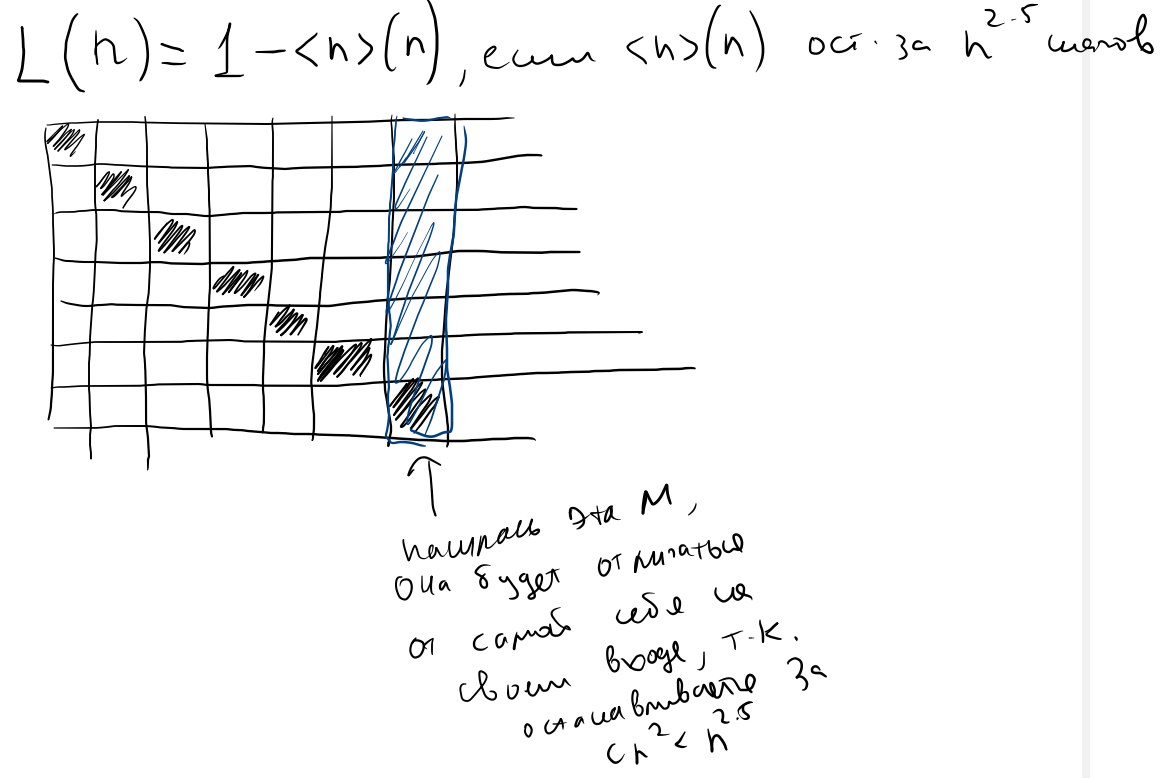
\includegraphics[scale=0.6]{diag.png}$$  
Рассмотрим язык $L = \{M | M$ отвергает $M$ за не более $|M|^{2.5}$  $\}$.
Пусть он решается квадратичной $M$ за $Cn^2$ шагов. Тогда давайте найдем эквивалентную ей $M'$ такую, что $|M'|^{2.5} > C|M'|^2$. Тогда получится, что $M'$ не равна себе же в строчке, соответствующей $M'$. \\
Как показать, что $L \in DTime[n^3]$? Давайте эмулировать МТ, которая работает $O(n^{2.5})$ с логарифмической задержкой.\\
Тогда получили нужный язык $L$. 
\end{proof}

\begin{defi}
$h : \N \rightarrow \N$ -- конструктивная по времени, если $n \rightarrow h(n)$ можно вычислить за $O(h(n))$ шагов на ДМТ.
\end{defi}

\begin{theorem}[Об иерархии по времени для детерменированных вычислений]
$f,g,h : \N \rightarrow \N$, $h$ -- конструктивная по времени.\\
$f(n) = o(h(n)), h(n)\log h(n) = o(g(n))$, тогда $DTime[f(n)] \subsetneq Dtime[g(n)]$.
\end{theorem}

\begin{proof}
Конструкция такая же, как и в предыдущем утверждении. Конструктивная функция нужна для будильника в МТ. $\log$ -- для эмуляции.
\end{proof}

\begin{prop}
$P \subsetneq EXP$.
\end{prop}
\begin{proof}
$P \subseteq DTime[2^n] \subsetneq DTime[2^{n^2}] \subseteq EXP$.
\end{proof}

\begin{note}
Доказательство не работает для НМТ, потому что мы не можем реверснуть ответ за такое же время.
\end{note}

\begin{sample}
$NTime[n^2] \subsetneq NTime[n^3]$.
\end{sample}
\begin{proof}
Определим для $M_i$ из перечисления всех НМТ отрезок $[n_i, n_i^{*}]$ так, что $n_i^{*} = 2^{n_i^{2.5}}$. \\
$n_{i+1} = n_i^{*}+1$.\\
$[n_1, n_1^{*}], [n_2, n_2^{*}], [n_3, n_3^{*}], \ldots$.\\
Определим язык $L$ так:
\begin{enumerate}
\item $L(n_i^{*}) = 1 - M_i(0^{n_i})$, если $M_i(0^{n_i})$ завершилось за менее чем $n_i^{2.5}$ шагов и 0 иначе.
\item $L(n) = M_i(0^{n+1})$ для $n_i \leq n < n_i^{*}$ 
\end{enumerate}
\begin{prop}
$L \notin NTime[n^2]$.
\end{prop}
Пусть это не так, тогда есть $M$, решающая $L$ за $Cn^2$. Возьмем такое ее вхождение, что $\forall n \in [n_i, n_i^{*}], n^{2.5} > Cn^2$. Тогда:
$$M(0^{n_i}) = L(0^{n_i}) = M(0^{n_i+1}) = L(0^{n_i+1}) = \ldots = L(0^{n_i^{*}}) \neq M(0^{n_i}) $$
так как все машины успеют отработать.
\begin{prop}
$L \in NTime[n^3]$. Разбираем случаи, если надо проэмулировать, то эмулируем, иначе нам нужно реверснуть выход недетерменированной машины. Мы можем сделать это за $2^{n_i^{2.5}} \cdot n_i^{2.5} < ((n_i)^{*})^3$.
\end{prop}
\end{proof}

\begin{theorem}[Об иерархии по времени для недетерменированных вычислений].
$f,g,h : \N \rightarrow \N$, $h$ -- конструктивная по времени.
$f(n) = o(h(n))$, $h(n+1) = o(g(n))$, тогда $NTime[f(n)] \subsetneq NTime[g(n)]$.

\begin{prop}
$NP \notin NEXP$.
\end{prop}
\begin{proof} аналогично детерменированному случаю.\end{proof}

\end{theorem}

\section{Билет 10}	
\begin{defi}[Модель вычислений с ограничением по памяти.]
 МТ с дополнительной лентой входа, она read-only, также по ней нельзя уйти правее первого пробела. Также есть лента выхода, по которой нельзя двигаться влево, а только выдавать очередной символ ответа. Затраченная память -- максимальный уход вправо на какой-то из рабочих лент.
\end{defi}

\begin{defi}
$DSpace[f(n)]$ -- класс языков, которые принимают ДМТ, использующие $O(f(n))$ памяти. $NSpace[f(n)]$ -- то же самое, но для НМТ.
\end{defi}

\begin{defi}
$PSPACE = \cup_{c>0} DTime[n^c]$, $NPSPACE = \cup_{c>0} NTime[n^c]$.
\end{defi}

\begin{defi}
$L = LOGSPACE = DSPACE[\log(n)]$, $NL = NSPACE[\log n]$.
\end{defi}

\begin{prop}
$\forall s(n)$ : $DTime[s(n)] \subseteq DSpace[s(n)] \subseteq NSpace[s(n)]$.
Причем первое включение работает лишь для некоторых моделей вычислений. В частности, для МТ.
\end{prop}

\begin{defi}
$S : \N \rightarrow \N$ -- конструктивная по памяти, если $1^{S(n)}$ можно вывести за $O(S(n))$ памяти.
\end{defi}

\begin{note} Для хороших функций выполняется также иерархия по памяти. То есть, например, известно, что $DSpace[n^2] \subsetneq DSpace[n^3], NSpace[n^2] \subsetneq NSpace[n^3]$.\\
(Смотри $TCS30, TCS31$).
\end{note}

\begin{theorem}
$s(n)$ -- конструктивная по памяти и $s(n) \geq \log n$. Тогда 
$$NSpace[s(n)] \subseteq DTime[2^{O(s(n)}] = \cup_{c>0} DTime[2^{cs(n)}]$$.
\end{theorem}
\begin{proof}
Для доказательства используется идея с графом конфигураций. Конфигурация МТ это набор параметров:
\begin{enumerate}
\item Положение головок на всех лентах
\item Содержание рабочих лент
\item Состояние
\end{enumerate}
Проблема выяснения того, принимает ли МТ вход $x$ может быть рассмотрена как проблема выяснения существования пути в графе конфигураций.  
 Поймем, сколько есть конфигураций:\\
$n \cdot (C s(n))^k$ -- положение головок, $2^{c' s(n) k}$ -- содержимое рабочих лент. Если $s(n) \geq \log n$, то это число есть $2^{O(s(n))}$. В таком случае мы можем сгенерировать такой граф и проверять наличие пути полиномиальным алгоритмом. Получится время работы $poly(2^{O(s(n))}) = 2^{O(s(n))}$. \\
Зачем пользовались конструктивностью функции по времени? Для того чтобы сгенерировать конфигурацию нужно отмерить максимальную длину конфигурации и дальше уже перебирать все возможные строчки. Поэтому хочется уметь отмерить за нормальную память. \\
То есть итоговый алгоиртм такой: по $M, x$ строим граф конфигураций и ищем путь из $K_0$ в $K_{accept}$. Можно сделать одно состояние $K_{accept}$, попросив МТ стирать все рабочие ленты перед тем как завершиться. Так мы унифицируем конечные состояние, но, очевидно, не изменим вычислительную мощь ($:)$).
\end{proof}

\begin{prop}.
\begin{enumerate}
\item $NSPACE \subseteq EXP$
\item $NP \subseteq EXP$  
\end{enumerate}
\end{prop}

\begin{theorem}[Савич]
$s(n)$ -- конструктивная по времени и $s(n) \geq \log n$, тогда $NSpace[s(n)] \subset DSpace[s(n)^2]$.
\end{theorem}
\begin{proof}
Все сводится к тому, чтобы по графу понять, есть ли в нем путь от вершины до другой за память $s(n)^2$, где $s(n)$ -- память рассматриваемой НМТ. Воспользуемся предикатом $PATH(u,v,i)$ -- есть ли путь от $u$ до $v$ длины не более $2^{i}$ и рекурсивным перебором. 
\end{proof}

\begin{prop}
$NPSPACE = PSPACE$
\end{prop}
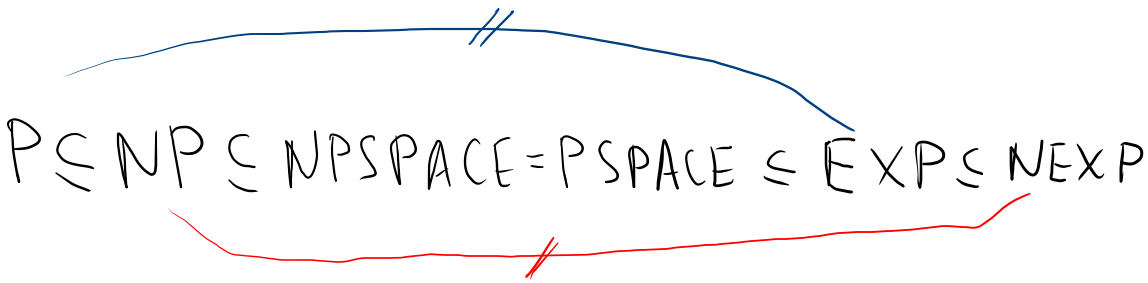
\includegraphics[scale=0.6]{hierarchy1.png}

\section{Билет 11}
Рассмотрим кванторные пропозициональные формулы: $Q_1 x_1, \ldots, Q_n x_n \ph(x_1, \ldots, x_n)$. Язык таких истинных формул это $TQBF$. Понятно, что $SAT \leqp TQBF$ просто дописываниям ко всем переменным квантора существования.\\
\begin{prop}
$TQBF$ лежит в $PSPACE$ 
\end{prop}
Действительно, можно просто сделать перебор рекурсивно и проверить выполнимость.

\begin{prop}
$TQBF$ -- полный в классе $PSPACE$.
\end{prop}
\begin{proof}
Берем граф конфигураций. Хотим записать формулу $PATH(K_0, K_{accept}, cp(n))$. (время работы не более $2^{cp(n)}$, так как иначе все зациклится).\\
Будем записывать при помощи следующего выражения: \\
$PATH(u, v, i) = \exists z \forall A, B ((A=u, B=z) \vee (A=z, B=v)) \rightarrow PATH(A, B, i-1)$, тогда мы сможем записать всё за полиномиальное количество бит. Остаются детали, как записать в виде формулы утверждения вида $PATH(u, v, 0)$. Мы можем с помощью полиномиального алгоритма проверить такой предикат. \\
Еще нужно подумать о том, как записать равенство конфигураций, это можно сделать просто побитово.
\end{proof}

\begin{note}
Выяснение вопроса детерменированной победы в конечных играх -- задача из $PSPACE$, так как ее можно записать в $TQBF$ в виде $\exists step_{1,1} \forall step_{2,1} \exists step_{1,2} \ldots Q(..)$, что означает, что есть ход первого игрока, что при любом ходе второго есть ход первого и тд, что первый игрок выиграл.
\end{note}

\section{Билет 12}
\begin{defi}[Логарифмическое сведение]
$A \leql B$, если существует $p$, вычислимая с использованием логарифмической памяти такая что $x \in A \Longleftrightarrow p(x) \in B$.
\end{defi}

\begin{prop}[Свойства лог сведений]
\begin{enumerate}
\item $A \leql B \Rightarrow A \leqp B$.
\item $A \leql B, B \leql C \Rightarrow A \leql C$.
\item $A \leql B, B \in L \Rightarrow A \in L$.
\end{enumerate}
\end{prop}
Чтобы доказать эти утверждения нужна лемма.
\begin{prop}
$f, g$ -- вычислимые с логарифмической памятью. Тогда $f \circ g$ тоже вычислима с логарифмической памятью. 
\end{prop}
\begin{proof}
Будем вычислять $f(g(x))$, когда для вычисления $f$ будет требоваться очередной бит входа, будем вычислять $i$-тый бит выхода $g(x)$ заново и ждать пока выведется бит под номером $i$. 
\end{proof}
$L \in NL$, а вот есть ли равенство -- открытый вопрос.
\begin{defi}[Определение NL через систему доказательств]
У нас появляется лента для подсказки, по которой можно двигаться только вправо (потому что НМТ не может записывать результат выбора на ленту). Это задает такой же класс языков, это можно видеть также как мы видели для разных определений $NP$.
\end{defi}
\begin{defi}
$DPATH = \{(G, u, v) |$ в ор. графе $G$ есть путь $u \rightarrow v$ $\}$. 
\end{defi}
$DPATH \in NL$, подсказкой является собственно путь. Нужно проверить, что первая вершина в нем есть $u$, последняя $v$ и что есть ребро между соседними, это можно сделать за $\log$ памяти.

\begin{theorem}
$DPATH$ -- $NL$ полный (относительно $\leql$).
\end{theorem}
\begin{proof}
пусть $A \in NL$, $M$ -- нмт, решающая $A$. Сведение будет следующим. Оно будет генерировать конфигурации, которые составляют максимум $\log$ памяти и выводить ребра между ними, то есть строить граф конфигураций. Далее выведем начальное и конечное состояние и это и будет искомый инстанс задачи $DPATH$.
\end{proof}

\begin{note}
Неизвестно, лежит ли $DPATH$ в $L$, или нет.
\end{note}

\begin{theorem}
$\overline{DPATH} \in NL$
\end{theorem}

\begin{proof}
Нам нужно сертифицировать, что между $s, t$ нет пути, причем сделать такое доказательство, которое можно читать слева направо и использовать логарифмическую память. \\
$U_i$ -- множество вершин, до которых есть путь от $s$ длины не более $i$. \\  
\begin{enumerate}
\item для $v$ можно сертифицировать, что $v \in U_i$, сертификат -- просто путь, как в языке $DPATH$.
\item если известно $|U_{i-1}|=k$, то можно сертифицировать, что $u \notin U_i$. Для этого предоставим список вершин из $U_{i-1}$ с сертификатами, что они действительно оттуда. Причем список будет у нас возрастающим, чтобы не было повторяющихся вершин. Проверим, что там правильное число вершин + нет вершины $u$ и также нет ребра между вершинами из списка и $u$. 
\item если известно $|U_{i-1}|=k$, то можно сертифицировать, что $|U_i| = t$. Просто для каждой вершины напишем одно из двух, либо сертификат того, что она лежит в $U_{i}$, либо сертификат того, что не лежит, при условии $|U_{i-1}|=k$.
\item Таким образом мы можем сертифицировать, что размер $U_{n-1}=k$ и что $t \notin U_n$. 
\end{enumerate}
\end{proof}

\begin{defi}[coЯзык]
$X$ -- класс языков. Тогда $coX = \{ \Sigma^* \setminus L | L \in X \}$. 
\end{defi}

\begin{note}
Как мы уже видели, $NP = coNP$ -- неизвестно.
\end{note}

\begin{theorem}
$s(n) \geq \log n$ -- конструктивная по памяти. Тогда $NSpace[s(n)]=coNSpace[s(n)]$.
\end{theorem}
\begin{proof}
$A \in NSPACE[s(n)]$, хотим показать, что $A \in coNSpace[s(n)] \Longleftrightarrow \overline{A} \in NSpace[s(n)] $. Причем, если покажем это, то автоматически последует равенство, так как для $A \in coNSpace[s(n)]$ надо показать, что $\overline{A} \in Nspace[s(n)]$, тогда из той стрелочки, которая описана это последует.\\
Рассмотрим $M$ -- НМТ, которая распознает $A$ с памятью $cS(n)$. $x \in \overline{A} \Longleftrightarrow x \notin A \Longleftrightarrow$ в графе конфигураций $G_x$ из $K_0$ нет пути в $K_{accept}$.\\
Сертификатом будет тот же самый, сертификат, что и был в теореме выше. Размер графа конфигураций будет $2^{O(s(n))}$, тогда нам потребуется $O(s(n))$ памяти, чтобы проверить сертификат. Причем граф строить полностью не надо, нужно всего лишь уметь проверять, есть ли некоторые ребра в нем. 
\end{proof}
\begin{note}
Выяснили на нынешний момент следующую картинку:\\
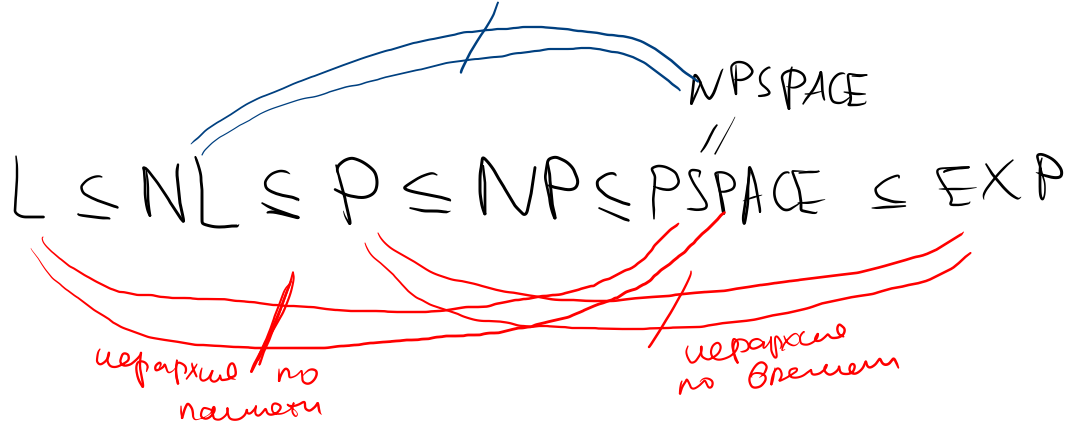
\includegraphics[scale=0.5]{hierarchy2.png}
\end{note}

\section{Билет 13}
\begin{defi}
Определение классов $\Sigma^P_0, \Sigma^P_1, \ldots$, а также $\Pi^P_0, Pi^P_1$.
\end{defi}
Интуиция про $NP, coNP$ и $\Sigma^P_1, \Pi^P_1$.\\
Можно развернуть определение:
$\forall x, x \in L \Longleftrightarrow \exists y_1 |y_1| \leq p(|x|) \forall y_2 , \ldots, y_i Q(x_, y_1, \ldots, y_i)$.
\begin{defi}
$PH = \cup_{i\geq0} \Sigma^P_i$
\end{defi}
\begin{prop}[Свойства полиномиальной иерархии].
\begin{enumerate}
\item $\Sigma^P_i \cup \Pi^P_i \subseteq Sigma^P_{i+1} \cap Pi^P_{i+1}$.
\begin{proof}
Добавляем фиктивные переменные и кванторы.
\end{proof}
\item $PH = \cup_{i\geq 0}Pi^P_i$.
\item $\Sigma^P_i = co\Pi^P_i$
\item $\Sigma^P_i = \Pi_i^P \Rightarrow PH = \Sigma^P_i$.
\begin{proof}
Доказательство индукцией по $j \geq i$, что $\Sigma^P_j = \Pi^P_j$. Используйте равенство предыдущего уровня для объединения кванторов в один.
\end{proof}
\item $\Sigma^P_i$ и $\Pi^P_i$ замкнуты относительно $\leqp$. 
\begin{proof}
Легко видеть, что надо просто взять вычислимый $Q$ из определения и попросить его использовать сведение чтобы охарактеризовать нужным образом язык. 
\end{proof}
\item
Если в $PH$ есть полный язык, то полиномиальная иерархия схлопывается. 
\begin{proof}
Просто все языки, начиная с уровня, на котором лежит полный, будут лежать в этом же уровне.
\end{proof}
\item 
Теперь введем полные языки на уровнях иерархии. Пусть $\Sigma SAT$ это язык, в котором лежат истинные формулы вида $\exists x_1 \forall x_2 \exists x_3, ..., x_i Q(x_1, \ldots, x_i)$, где $x_i$ -- возможно вектор значений. Аналогично, только с противоположными кванторами определяется $\Pi_i$. 
\begin{prop}
при $i\geq 1$ выполняется то, что 
$\Sigma_i SAT$, $\Pi_i SAT$ полны в соответствующих классах на $i$-том уровне полиномиальной иерархии.
\end{prop}
\begin{proof}
Покажем про $\Sigma_i SAT$. В начале то, что он лежит в $\Sigma_i^P$. Характеристика его такова: так как мы не знаем точно сколько там переменных внутри векторочков, то будем в каждый блок класть столько переменных, чтобы нам хватило. То есть, характеристика следующая: $\exists x_1, |x_1| = |\ph|, \forall x_2 |x_2| = |\ph|, \ldots, x_i : A(\ph, x_1, \ldots, x_i)$. $A$ -- просто полиномиальный алгоритм, который берет и подставляет из наших блоков переменные в $\ph$ и проверяет то, что она истинна. Таким образом показали включение.\\
Теперь полнота. Возьмем некоторый язык $L \in \Sigma^P_i$. Его характеризация имеет вид: $\exists y_1, |y_1| = p(|x|), \ldots, y_i Q(x, y_1, \ldots, y_i)$. Можно в характеризации сделать все игрики фиксированной длины (в отличии от того что у нас раньше была оценка сверху на длину), так как можно допихать нулей в случае чего. \\
$Q(x, y_1, \ldots, y_i)$ -- какой-то полиномиально вычислимый предикат. Давайте переделаем его в схему. Это получится, так как $y_1, \ldots, y_i$ и $x$ имеют фиксированную полиномиальную длину. Теперь переделаем схему в формулу при помощи введения дополнительных переменных для всех узлов схемы и обеспечивания соответствующих равенств. Получится формула вида $\exists t \ph(x, y_1, \ldots, y_n)$. Если вдруг нам и нужен был квантор существования в конце ($i$ -- нечетно), то мы уже победили. Иначе воспользуемся трюком с существованием для отрицания и получим запись с квантором всеобщности. Тогда этот квантор можно совместить с последним квантором из характеризации $L$. 

\end{proof}
\end{enumerate}
\end{prop}

\section{Билет 14}
\begin{theorem}
$\Sigma_{i+1}^P = NP^{\Pi_i SAT}$
\end{theorem}
\begin{proof}
.\\$\subseteq:$ $L \in \Sigma_{i+1}^P$ тогда есть следующая характеризация $\exists L' \in \Pi_i^P, \forall x \in L \Leftrightarrow \exists y \in \{0, 1\}^{p(|x|)}, (x, y) \in L'$. Тогда пусть наша НМТ генерирует этот $x$, потом делает запрос к оракулу при помощи сведения $(x, y)$ к $\Pi_i SAT$. \\
$\supseteq:$ пусть $L \in NP^{\Pi_i SAT}$ и его решает НМТ $M$ за $p(n)$ с использованием оракула $\Pi_i$. \\
$x \in L \Longleftrightarrow \exists z \in \{0,1\}^{p(n)}, T_1(x, z) \wedge T_2(x, z) \wedge T_3(x, z) $, где
\begin{enumerate}
\item $z$ отвечает за недетерменированные выборы НМТ и ответы оракулов.
\item $T_1(x, z)$ проверяет, что мы действительно принимаем $x$ действуя согласно строке $z$
\item $T_2(x, z)$ проверяет, правда ли, что оракул дал верные положительные ответы. Все вопросы к оракулу выглядит как формулы вида: $\forall x_1, \ldots, x_k \ph(x_1, \ldots, x_k)$. Тогда давайте $T_2$ будет выглядеть так: $\forall r_1 \in \{0,1\}^{p(n)^2}, \ldots r_k \in \{0, 1\}^{p(n)^2} R(x, z, r_1, \ldots, r_k)$, где $R$ поблочно подставляет переменные во все формулы, про которые спрашивал наш алгоритм у оракула и проверяет истинность.
\item $T_3$ проеряет отрицательные ответы оракула. Для того, чтобы проверить, что $\ph$ ложна -- нужно проверить, что истинно отрицание $\ph$, то есть, что $\exists x_1, \ldots, x_k !\ph(x_1, \ldots, x_k) = 1$. Тогда давайте запишем характеристику следующим образом: 
$\exists x_1 \in \{0,1\}^{p(n)^2}, \ldots, x_k \in \{0, 1\}^{p(n)^2} T'(x, z, x_1, \ldots, x_k)$ и $T'$ выдает 1 тогда и только тогда, когда все формулы обнулились. 
\end{enumerate}
Теперь вынесем кванторы независимо из $T_1, T_2$. Получится нужное чередование. 
\end{proof}

\section{Билет 15}
\begin{defi}[Вычисления с неравномерной подсказкой]
Языки, принимаемые МТ с неравенномерной подсказкой длины $K(n)$ ($P / K(n)$) это такие языки, для которых существует $M$ -- МТ с лентой для подсказки и $\alpha_n$ -- последовательность подсказок длины $\leq K(n)$ такие, что МТ понимает, лежит ли $x$ в $L$, используя подсказку $\alpha_{|x|}$.
\end{defi}
\begin{note}
$P/1$ содержит неразрешимые языки. 
\end{note}

\begin{prop}
$\cup_{c} P / n^c = P / poly$.
\end{prop}
\begin{proof}.\\
$\subseteq$: давайте переделаем МТ в схемы, потом встроив туда подсказку. Получим последовательность схем. \\
$\supseteq$: в качестве подсказки возьмем схему.
\end{proof}
          
\begin{theorem} Существует функция $f : \{0, 1\}^n \rightarrow \{0, 1\}$ такая, что она не вычислима схемой размера менее $2^n / 10^n$.
\end{theorem}

\begin{proof}
Схему размера $T$ можно задать за не более чем $4T \log T$ битов. Тогда таких схем не более $2^{4 T \log T}$. Пусть $T < 2^n / 10n$. Тогда покажем, что $2^{4 T \log T} < 2^{2^n}$. Нужно показать: $4 T \log T < 2^n$, действительно: $4 T \log T < 4 2^n/(10n) \log(2^n/10n) < 4 * 2^n / 10 < 2^n$. 
\end{proof}

\section{Билет 16}
\begin{theorem}[Карп-Липтон]
Если $NP \in P/poly$, то полиномиальная иерархия схлопывается на втором уровне.
\end{theorem}
\begin{proof}
За счет того, что мы умеем сводить задачи распознавания к задачам поиска, у нас существует и семейство схем, которое выдает выполняющие наборы для схем. Пусть это семейство $C_n$. Причем пусть размеры ограничены полиномом $p(n)$\\
Хотим показать, что $\Sigma^P_2 = \Pi^P_2$. Нам хватит показать, что $\Pi_2 SAT$ лежит в $\Sigma^P_2$, так как это $co$ языки друг друга.\\
Что у нас лежит в $\Pi_2 SAT$? Истинные формулы вида $\forall x \exists y Q(x, y)$. Давайте попробуем написать для этого языка $\Sigma^P_2$ характеристику.\\
$\ph \in \Pi_2 SAT \Longleftrightarrow \exists C_1, \ldots C_{|\ph|} \forall z \in \{0,1\}^{|\ph|} T_{z} (C_{|T_{z}|} (T_z)) = 1 $. Мы легко можем проверить последний предикат за полиномиальное время. Причем из того, что $NP \in P/poly$ будем существовать нужный набор схем в случае, если формула действительно лежит в языке.
\end{proof}

\section{Билет 17}
\begin{theorem}[Первая теорема Каннана]
$PH$ не лежит в $Size[n^k]$ ни для какого $k$.
\end{theorem}
\begin{proof}
Давайте построим язык, который будет содержаться в $PH$, но при этом не решаться схемами размера $n^k$. \\
Посмотрим на булевы функции от $(k+1)\log n$ переменных. Тогда по теореме про существование сложной фунцкии, среди таких функций найдется функция, схемная сложность которой более $2^{(k+1)\log n}/10n = \frac{n^{k+1}}{10(k+1)\log n}$, что больше $n^k$ при больших $n$.\\
Будем с помощью кванторов задавать первую такую функцию. Скажем, что $x \in L \rightarrow \forall f (\forall C |C| \leq n^k \Longleftrightarrow \exists x C(x) \neq f(x)), \forall g (g \prec f, \exists C |C| \leq n^k \forall x C(x) = g(x)) \rightarrow f(x) = 1$. Мы сможем проверить предикат лексикографической меньшести и равенства функции, так как функцию из $(k+1)\log n$ битов можно задать таблицей истинности полиномиального размера. 
\end{proof}

\begin{theorem}[Вторая теорема Каннана]
Уже в $\Sigma_2^P \cap \Pi_2^P$ есть язык, который не распознается семейством полиномиальных схем.
\end{theorem}
\begin{proof}
Пусть это не так. Тогда $NP \in \Sigma_2^P \cap \Pi_2^P \leq P/poly$, но тогда из теоремы Карпа-Липтона получим, что полиномиальная иерархия схлопывается на 2 уровне и $PH = \Sigma_2^P$, но это противоречие с первой версией теоремы Каннана.  
\end{proof}

\section{Билет 18}
\begin{defi}
Семейство схем $C_n$, имеющих $n$ входов, называется равномерным, если есть логарифмическая по памяти машина Тьюринга, генерирующая нам по входу $1^n$ выход $C_n$.
\end{defi}

\begin{theorem}
Класс языков, распознающихся семейством равномерных схем есть класс $P$.
\end{theorem}
\begin{proof}
Если распознается семейством равномерных схем, то давайте будем генерировать схему и проверять на наличие. Будет работать за полином, потому что алгоритм, генерирующий схему, лежит в $L$. Теперь заметим, что наш алгоритм, который переводит МТ в схему -- тоже логарифмический. Потому что ему для построения нужно было выписывать какие-то ячейки на одном уровне и при этом добавлять ребра между некоторым константным количеством соседних ячеек, тут нет сильно затратных по памяти операций.
\end{proof}

\begin{note}
Часто считают, что задача поддается эффективному распараллеливанию, если ее можно решить на $poly(n)$ процессоров за $\log n$, где $n$ -- длина входа.
\end{note}

\begin{note}
Если смогли распараллелить на $n$ процессорах, то можно поделить это число на какую-нибудь константу, степень распараллеливания тоже поделится примерно на константу.
\end{note}
Можно представлять себе распараллеленные вычисления как схему малой глубины.

\begin{defi}
$NC = \cup_{i>0} NC^i$. \\
$L \in NC^i$ тогда и только тогда, когда существует последовательность равномерных схем $C_n$, распознающих $L$ и глубина $C_n \leq O(\log^i n)$.
\end{defi}
\begin{note}
$NC \subseteq P$, потому что это множество слабее, чем то, которое равно $P$: мы добавили ограничение на глубину схемы. При этом открытым вопросом является равенство $NC$ и $P$.
\end{note}
В каких-то $P$--подобных классах интересно рассматривать $\leql$ сведения, потому что по Карпу и так почти все сводится друг к другу тривиально.

\begin{defi}
$Circuit-Value = \{(C, x)$ $C$ -- булева схема, $C(x)=1$ $\}$ является $P$-полным относительно $\leql$ сведений. 
\end{defi}
\begin{proof}
Понятно, что этот язык лежит в $P$. Как свести? Давайте построим по МТ схему как обычно логарфмическим алгоритмом.
\end{proof}

\begin{note}
Попытка объяснения про задачу, почему она не распараллеливается могла бы быть такой: давайте сведем ее к $Circuit-Value$. Поскольку, неизвестно равны ли $P$ и $NC$, то если бы это было не так, то попытка объяснения бы сработала.
\end{note}

\begin{prop}
$DPATH \in NC^2$, если граф задан матрицей смежности.
\end{prop}
\begin{proof}
Чтобы понять, есть ли путь из вершины в другую, надо $k$ раз возвести в квадрат матрицу смежности, где $k = \lceil \log n \rceil$. Тогда давайте строить схему, делающую это. Там будет $k$ возведений матрицы в квадрат. Причем каждое возведение добавляет в схему $O(\log n)$ высоты, что нетрудно видеть, посмотря на пример ниже. \\
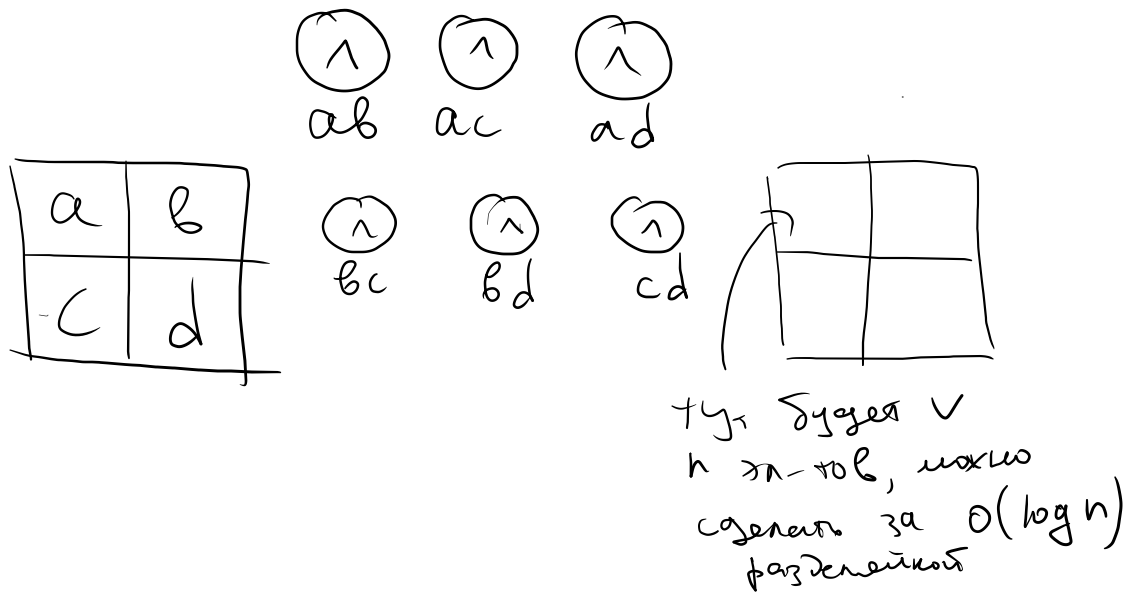
\includegraphics[scale=0.6]{matrix_scheme.png}\\
Теперь надо взять элемент $(s,t)$ у этой матрицы. \\
Покажем схему, которая поможет выбрать $i$-тый элемент массива, если $i$ задано в двоичном виде. Основываемся на идее, что если старший бит $i$ равен 1, то брать надо из правой половины, иначе -- из левой. Построим для половинок схемы на $n-1$ бите и так далее. Получится глубина $O(\log n)$, пример на рисунке для $n=4$:\\
$$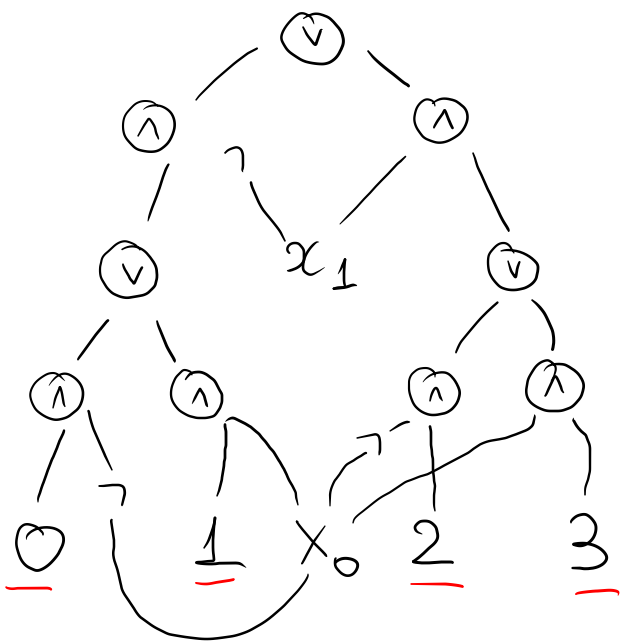
\includegraphics[scale=0.6]{scheme_for_choose.png}$$
Тогда выберем из каждой строчки элемент $t$, а дальше из всех выбранных выберем элемент $s$, получится схема глубину $2\log n$. Таким образом, построили схему нужной глубины.\\
Важно, что все схемы, которые мы тут обсудили можно сгенерировать с использованием логарифмической памяти. Проверять это довольно нудно, но видно, что, например в последней схеме, нужно просто бежать по уровням и выводить ребра с элементами с фиксированными номерами, получающимися по какой-нибудь формуле типа $2i$, незачем хранить всё целиком.
\end{proof}
\begin{prop}
Классы $NC^i$ при $i \geq 2$ замкнуты относительно логарифмических сведений. 
\end{prop}
\begin{proof}
Доказательство очень глиняное. Пусть есть $B \in NC^i, A \leql B$, $f$ -- сведение. Тогда хотим сделать следующее: в начале вычислять сведение при помощи схемы глубины $\log^2$, а дальше считать уже спокойненько функцию схемой для языка $B$. Будем считать сведение так: посчитаем отдельно каждый его бит. Всего будет какой-то полином битов. Нам нужно проверить, что при нашем входе сведение выдаст на $j$-тый бит, бит 1. Давайте возьмем МТ, которая такая же как сведение, но, она еще принимает бит, который надо выдать и в конце приходит в состояние $q_yes$ или $q_no$ в зависимости от значения этого бита. Далее переделаем всё это в схему при помощи предыдущего утверждения и графа конфигураций.  
\end{proof}
\begin{note}
Вспомним, что $DPATH$ -- $NL$ полный. Отсюда получается, что $NL \subseteq NC^2$.
\end{note}
\begin{theorem}
$NC^1 \subseteq L \subseteq NL \subseteq NC^2$
\end{theorem}
\begin{proof}
Из всего вышесказанного, остается показать лишь $NC^1 \subseteq L$. Возьмем какой-нибудь язык $L \in NC^1$. Хотим решить его за логарифмическую память, сделаем следующие действия по $x$:
\begin{enumerate}
\item Построим схему, решающую данный язык с помощью алгоритмы из $NC^1$
\item Переделаем схему в формулу
\item Вычислим формулу с помощью рекурсии
\end{enumerate}
Если покажем, что каждое действие можно сделать за $O(\log n)$ памяти, то можно будет и всё сделать за такую память, так как композиция функцих, вычислимых за $O(\log n)$ памяти тоже функция такого вида.
\begin{enumerate}
\item Работаем тут за $O(\log)$ памяти, так как нужно просто применить алгоритм, который нам предоставляет схему за такую память из $NC^1$, подав ему на вход нужное число единиц.
\item Понятно, что из схемы высотой $O(\log)$ получится формула тоже не более чем такой высоты. Будем копировать вершины, построив что-то вроде двоичного бора на нашей схеме и всякий раз доходя до какой-то вершины, копируя её и выдавая номер, соответствующий пути в боре. Нам понадобится $O(\log)$ памяти, так как по сути нужно хранить нынешний путь в виде числа (можно изначально задать соответствие вершин и таких путей, чтобы понимать, в какой мы сейчас вершине). Подробнее на рисунке:\\
$$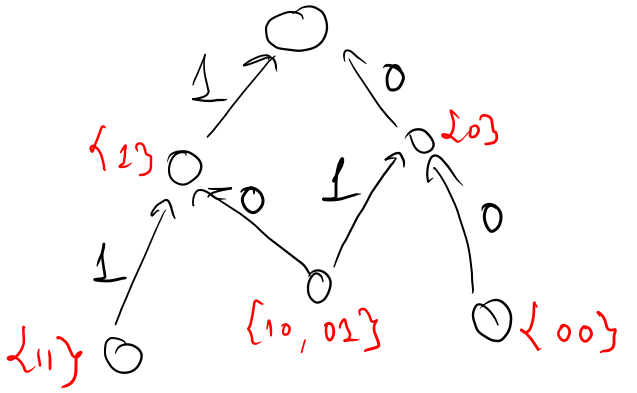
\includegraphics[scale=0.7]{scheme_to_formula.png}$$	
\item Вычисление формулы занимает $O(\log n)$ памяти, примерно по тому же, почему и в предыдущем пункте.
\end{enumerate}
\end{proof}

\section{Билет 19}
\begin{defi}
Какая-то интуиция коммуникационной сложности + пример про делимость и определение $EQ$.
\end{defi}
\begin{defi}[Коммуникационный протокол]
Это дерево, в котором в каждой вершине либо что-то передает Алиса, либо Боб. То есть там написана функция Алисы из ее входа в $\{0, 1\}$, либо Боба. История взаимодействия учитывается, так как везде может быть своя функция.\\
$$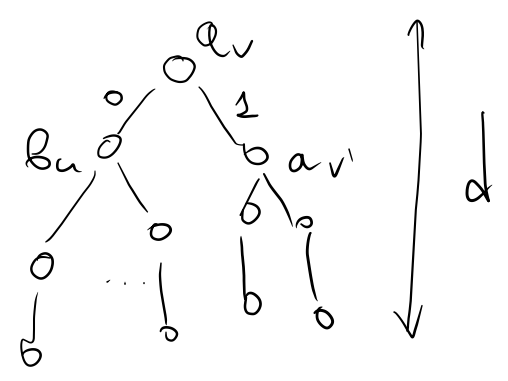
\includegraphics[scale=0.7]{communication_protocol.png} $$
\end{defi}
\begin{defi}
Коммуникационная сложность протокола -- его высота. Обозначается как $D(\Pi)$. Коммуникационная сложность функции это минимальная коммуникационная сложность протокола, вычисляющего её. Обозначется аналогично. 
\end{defi}
$M_f$ -- матрица для $f : X \times Y \rightarrow Z$, если $M_{i,j} = f(i, j)$. Комбинаторный прямоугольник -- множество $X' \times Y'$ для некоторых $X' \subseteq X, Y' \subseteq Y$. Комбинаторный прямоугольник назовем одноцветным тогда и только тогда, когда все элементы матрицы, соответствующие ему равны попарно. \\
Заметим, что каждый ход в протоколе разбивает какой-то прямоугольник на еще несколько в зависимости от значения функции, а листья протокола соответствуют как раз одноцветным прямоугольникам, так как в них значения определены корректно и однозначно.\\
Отсюда получается: 
\begin{prop}
Если в протоколе для $f$ есть $k$ листьев, то $f$ можно разбить на $k$ одноцветных прямоугольников.
\end{prop}
Другими словами, число листьев в протоколе $\geq$ минимальное число одноцветных прямоугольников, на которое можно разбить $M_f$. 	
\begin{theorem}
Сложность протокола $EQ$ есть $n+1$.
\end{theorem}
\begin{proof}
Очевидно, как сделать за $n+1$. Нужна оценка снизу. Будем доказывать при помощи подсчета одноцветных прямоугольников в матрице для $EQ$. Эта матрица это $E_{2^n}$. В ней никакие 2 единицы не могут принадлежать одному прямоугольнику. А значит, прямоугольников хотя бы $2^n+1$, что свидетельствует о том, что высота протокола будет $\geq n+1$. 
\end{proof}

\section{Билет 20}
Оказывается, что можно доказывать некоторые забавные вещи при помощи построенной конструкции.
\begin{theorem}
Для одноленточной МТ, рещающей язык палиндромов, выполнено $T \cdot S = \Omega(n^2)$, где $T$ -- время работы, $S$ -- затраченая память.
\end{theorem}
\begin{proof}
Возьмем такую МТ $M$. По ней построим коммуникационный протокол для вычисления $EQ$. Будем рассматривать строки $x0^ny^{rev}$, которые являются палиндромами тогда и только тогда, когда $x=y$. Пока МТ не вышла за самую правую перегордку, стоящую после искуственно добавленных нулей, Алиса будет эмулировать ее, а дальше отправит Бобу состояние ленты, а также состояние МТ. Далее также будет делать Боб, но наоборот, до момента, пока МТ не дойдет до самой левой перегородки после искуственно добавленных нулей. \\
Тогда сложность такого протокола равна $(O(1) + O(S(x0^ny^{rev})) \frac{T(x0^ny^{rev})}{n} \geq n + 1$, отсюда искомое неравенство. $n$ в знаменателе, так как между передачами проходит хотя бы $n$ действий МТ.
\end{proof}

\section{Билет 21}
\begin{defi}[Про отношения].
\begin{enumerate}
\item Отношением назовем множество троек $R \subseteq X \times Y \times Z$.
\item Отношение тотально, если $\forall x, \forall y, \exists z, (x,y,z) \in R$.
\item Функция $f$ реализует тотальное отношение, если $\forall x \in X, \forall y \in Y, (x,y,f(x,y)) \in R$.
\item Коммуникационный протокол для тотального отношения $R$ -- это коммуникационный протокол для какой-нибудь функции его реализующей.
\item Коммуникационная сложность тотального отношения -- глубина наимненьшего коммуникационного протокола для него.
\end{enumerate}
\end{defi}

\begin{defi}[Отношение Карчмар-Вигдерсон].
$f : \{0,1\}^n \rightarrow \{0, 1\}$. $f(x) = 0$, $f(y) = 1$. \\
$KW_f = \{ (x,y,z)\;|\;$ $f(x)=0, f(y)=1, x_i \neq y_i$ $\}$.
\end{defi}
\begin{prop}[Лемма Карчмар-Вигдерсон]
Если у булевой функции $f$ есть формула, вычисляющая ее с $l$ листьями, то есть коммуникационный протокол, который ее вычисляет с не более чем $l$ листьями. 
\end{prop}
\begin{proof}
В начале перенесем отрицания к листьями в формуле. Далее поддерживаем инвариант в каждой вершине, что у Алиса прообраз нуля функции, вычисляемой в этой вершине, у Боба -- прообраз единицы. В узлах, где последняя операция ИЛИ -- выбирать будет Боб -- ему надо пойти в единичное поддерево, а там где И -- Алиса. В конце в листьях как раз и будут отличающиеся биты, так как там вычисляются тривиальные функции.
\end{proof}
Другими словами, кол-во листьев в формуле $\geq$ минимальное количество листьев в протоколе для отношения Карчмар-Вигдерсон этой функции.

\section{Билет 22}
Теперь применим то, что было в предыдущих билетах. А именно, цепочку неравенств для булевой функции $f$:
$$\#min\_leafs\_in\_formula(f) \geq min\_height(KW_f) \geq min\_cnt\_monochrome(M_f)$$

\begin{prop}
$X,Y$ -- непересекающиеся подмножества $\{0, 1\}^n$, $C = \{(x,y)\;|\;x\in X, y\in Y,$ $x,y$ различаются ровно в одном бите $\}$. $M$ -- матрица на $X \times Y$. $\forall x \in X, y \in Y$ выполнено $M_{x,y} = $ бит различия $x, y$. Тогда $$T \geq \frac{|C|^2}{|X||Y|}$$ где $T$ -- минимальное число одноцветных комбинаторных прямоугольников, на которое можно разбить $M$.
\end{prop}
\begin{proof}
Пусть $R_1 \sqcup R_2 \sqcup \ldots \sqcup R_{T}$ -- разбиение $M$ на одноцветные прямоугольники. $m_i = |R_i \cap C|$. \\
Посмотрим на $R_i$, утверждается, что в нем нет двух элементов из $C$ в одной строке. Дейсвительно, все пары отличаются в одинаковом бите. Если ровно в одном, то не может быть такого, что такие пары две в строке, иначе у нас какой-то элемент написан дважды. Аналогично для столбцов. Отсюда выполняется $|R_i| \geq m_i^2$.
$$|C|^2 = (\sum_{i \in [T]} m_i)^2 \leq T \sum_{i \in [T]} m_i^2 \leq T |X| |Y| $$. Отсюда искомое неравенство. Использовали КБШ в оценке (представили как $1 \cdot m_i$).
\end{proof}

\begin{prop} Формула для $Parity_n$ имеет размер $\Omega(n^2)$.
Воспользуемся цепочкой неравенств выше. Для оценки самой правой величины в цепочке используем предыдущее утверждение. Возьмем $X = Parity_n^{-1}(0)$, $Y = Parity_n^{-1}(1)$. Тогда сколько есть для элемента из $X$ парных с ним таких, что они отличаются в одном бите из $Y$? Понятно, что все такие лежат в $Y$ и их $n$ штук. Тогда неравенство говорит нам, что $T \geq n^2$, что и хочется.
\end{prop}

\end{document}















